\documentclass{beamer}
\usepackage[utf8x]{inputenc}
\usepackage[ngerman]{babel}
\usepackage{amsmath}
\usepackage{amsfonts}
\usepackage{amssymb}
\usepackage{graphicx}
\usepackage{subfigure}
\author{Johannes Hackel und Falco Prescher}
\title{Bildverarbeitung mit OpenCL}

\usetheme{Ilmenau}
\useoutertheme{split}
\usecolortheme{rose}

\newcommand*\oldmacro{}%
\let\oldmacro\insertshorttitle%
\renewcommand*\insertshorttitle{%
  \oldmacro\hfill%
  \insertframenumber\,/\,\inserttotalframenumber}

\begin{document}

\begin{frame}
\titlepage
\end{frame}

\begin{frame}
\frametitle{Gliederung}
\tableofcontents
\end{frame}

\section{OpenCL}

\subsection{Allgemeines zu OpenCL}
\begin{frame}
\frametitle{Allgemeines zu OpenCL}
\begin{itemize}
\item Test
\end{itemize}
\end{frame}

\subsection{Grundlegender Aufbau eines OpenCL-Programmes}
\begin{frame}
\frametitle{Grundlegender Aufbau eines OpenCL-Programmes}
\begin{itemize}
\item Test
\end{itemize}
\end{frame}

\section{Vergleich von OpenCL mit CUDA}

\subsection{Unterstütze Plattformen}
\begin{frame}
\frametitle{Unterstütze Plattformen}
CUDA:
\begin{itemize}
\item NVIDIA-GPUs
\end{itemize}
OpenCL:
\begin{itemize}
\item alle Recheneinheiten die OpenCL unterstützt
\item CPUs, GPUs
\end{itemize}
\end{frame}

\subsection{Performance}
\begin{frame}
\frametitle{Performance}
CUDA:
\begin{itemize}
\item Hardware und Technologie vom gleichen Hersteller
\item gute Implementation
\item gute Leistung
\end{itemize}
OpenCL:
\begin{itemize}
\item von Plattform abhängig
\item Faktoren: Leistung, Implementation
\end{itemize}
\end{frame}

\subsection{API/Modell}
\begin{frame}
\frametitle{API/Modell}
\begin{itemize}
\item Modelle ähneln sich
\item Begriffsunterchiede
\item weitere Unterschiede
\end{itemize}
\end{frame}

\begin{frame}
\begin{center}
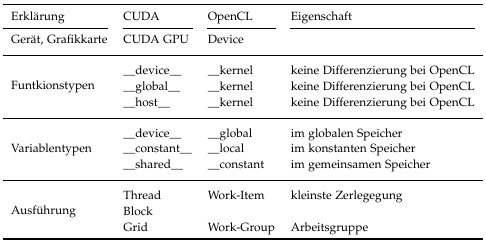
\includegraphics[width=10cm]{cuda_opencl_begriffe.png}
\newline Quelle: [1]
\end{center}
\end{frame}

\subsection{Entwicklungsaufwand}
\begin{frame}
\begin{center}
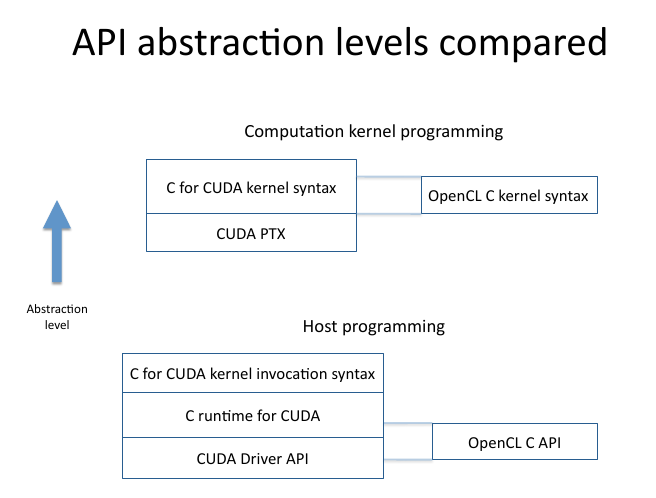
\includegraphics[width=9cm]{api_abstraction_level.png}
\newline Quelle: [2]
\end{center}
\end{frame}

\begin{frame}
\frametitle{Entwicklungsaufwand}
OpenCL:
\begin{itemize}
\item API mit geringer Abstraktion
\item verschiedene Debugging-Möglichkeiten je Plattform
\item guter Debugger(cross-plattform): gDEBugger
\item verschieden Geräte: unterschiedliche Implementation
\end{itemize}
CUDA:
\begin{itemize}
\item geringe und hohe Abstraktion
\item viele Bibliotheken
\item guter Debugger durch CUDA-SDK
\end{itemize}
\end{frame}

\section{Bildverarbeitung}

\subsection{Allgemeines zu Bildverarbeitung mit OpenCL}
\begin{frame}
\frametitle{Allgemeines zu Bildverarbeitung mit OpenCL}
\begin{itemize}
\item Test
\end{itemize}
\end{frame}

\subsection{Kantenerkennung von Bildern in OpenCL}
\begin{frame}
\frametitle{Kantenerkennung von Bildern in OpenCL}
\begin{itemize}
\item Test
\end{itemize}
\end{frame}

\begin{appendix}
\begin{frame}
\frametitle{Quellen}
\begin{enumerate}
\item \url{ftp://ftp.informatik.uni-stuttgart.de/pub/library/medoc.ustuttgart_fi/DIP-3178/DIP-3178.pdf}
\item \url{https://wiki.aalto.fi/download/attachments/40025977/Cuda+and+OpenCL+API+comparison_presented.pdf}
\end{enumerate}
\end{frame}
\end{appendix}

\end{document}